% 골든 · 유형 6 그리드·색칠 넓이 (해설용 · 풍부)
% 세션 75 신설 · 와부고 스타일 도입
% [[feedback_wabuko_graph_standard]] 5대 원칙 준수 · 참조 pdf "문제에 넣을 그림 (수정)" [해설에 넣을 그림]
%
% 목적 : 두 곡선 사이 영역의 넓이 풀이 (답지)
%   - 해설용 : 문제용 + 눈금·점선 grid·영역 색칠·영역 라벨 (A·B)
%   - 격자점 개수 등의 문항에서 학생이 시각 이해
%
% 색칠 표준 :
%   - A 영역 : 노랑 계열 (`fill=yellow!30`) · 파스텔
%   - B 영역 : 파랑 계열 (`fill=cyan!30`) · 파스텔
%   - 두 영역 위 라벨 : "A", "B" · 굵은 서체

\begin{center}
\begin{tikzpicture}[scale=1.0]
  % ── 두 곡선 (해설 시각화 필수 · 색칠 앞에 정의)
  %   상단 : y = 36/(x+10) + 4 · 하단 : y = √x
  \begin{scope}
    \clip (0, 0) rectangle (5.7, 5);
    % 영역 A · 노랑 (하단 곡선 아래)
    \fill[yellow!30]
      plot[domain=0:5.7, samples=100] (\x, {sqrt(\x)}) --
      (5.7, 0) -- (0, 0) -- cycle;
    % 영역 B · 파랑 (두 곡선 사이)
    \fill[cyan!30]
      plot[domain=0:5.7, samples=100] (\x, {36/(\x + 10) + 4 - 3.6}) --
      (5.7, 0) plot[domain=5.7:0, samples=100] (\x, {sqrt(\x)}) -- cycle;
  \end{scope}

  % ── 축 (실효 0.7pt)
  \draw[-stealth, black, line width=0.7pt] (-0.5, 0) -- (6, 0) node[below, font=\scriptsize] {$x$};
  \draw[-stealth, black, line width=0.7pt] (0, -0.5) -- (0, 5) node[left, font=\scriptsize] {$y$};
  \node[font=\scriptsize, below left] at (0, 0) {$\mathrm{O}$};

  % ── 축 눈금 (해설용 신규 · 특징 좌표값)
  \foreach \x/\lb in {1/1, 2/4, 3/8, 4/16, 5/25} {
    \node[font=\tiny, below] at (\x, -0.02) {$\lb$};
  }
  \foreach \y/\lb in {1/1, 2/2, 3/3, 4/4} {
    \node[font=\tiny, left] at (-0.02, \y) {$\lb$};
  }

  % ── 점선 grid (해설용 신규 · 각 눈금에서 축까지 · 얇은 회색)
  \foreach \x in {1, 2, 3, 4, 5} {
    \draw[gray, line width=0.3pt, dash pattern=on 1pt off 1pt]
      (\x, 0) -- (\x, 4);
  }
  \foreach \y in {1, 2, 3, 4} {
    \draw[gray, line width=0.3pt, dash pattern=on 1pt off 1pt]
      (0, \y) -- (5.7, \y);
  }

  % ── 곡선 (색칠 위에 · 검정 실선)
  \draw[black, line width=0.5pt, domain=0:5.7, samples=100]
    plot (\x, {36/(\x + 10) + 4 - 3.6});
  \draw[black, line width=0.5pt, domain=0:5.7, samples=100]
    plot (\x, {sqrt(\x)});

  % ── 영역 라벨 (색칠 위 · 굵은 서체 · 중앙 배치)
  \node[font=\small\bfseries, black] at (2.5, 0.8) {$\mathrm{A}$};
  \node[font=\small\bfseries, black] at (2.5, 2.3) {$\mathrm{B}$};

  % ── 곡선 라벨 (프레임 안)
  \node[font=\scriptsize, anchor=west] at (2.5, 3.5) {$y=\dfrac{36}{x+10}+4$};
  \node[font=\scriptsize, anchor=west] at (4.5, 2.0) {$y=\sqrt{x}$};
\end{tikzpicture}
\end{center}

% === 문제용 대비 추가 요소 ===
% 1. \fill[yellow!30]·\fill[cyan!30] · 영역 색칠 (\clip으로 프레임 안 제한)
% 2. \foreach 축 눈금 라벨 (해설용 특징 좌표값)
% 3. \foreach 점선 grid (모든 눈금에서 곡선까지)
% 4. 영역 라벨 (A · B · 굵은 서체)
%
% === 사용 시 교체 대상 ===
% 1. 두 곡선 방정식·domain
% 2. 색칠 영역 정의 (\fill · \clip 조합)
% 3. 축 눈금 값 (\foreach \x/\lb in {...})
% 4. 점선 grid 좌표
% 5. 영역 라벨 위치·이름 (A·B)
%
% === 유지 대상 ===
% - scale=1.0
% - 색칠 파스텔 (yellow!30·cyan!30)
% - grid 점선 두께 0.3pt (곡선 방해 X)
% - 곡선을 색칠 위에 그림 (검정 실선이 색칠 위로 노출)
